\documentclass[12pt,a4paper]{article}

% Packages
\usepackage[utf8]{inputenc}
\usepackage[T1]{fontenc}
\usepackage{lmodern}
\usepackage[margin=2.5cm]{geometry}
\usepackage{graphicx}
\usepackage{hyperref}
\usepackage{listings}
\usepackage{xcolor}
\usepackage{booktabs}
\usepackage{amsmath}
\usepackage{amssymb}
\usepackage{tikz}
\usetikzlibrary{shapes.geometric, arrows, positioning, fit, backgrounds}
\usepackage{float}
\usepackage{enumitem}
\usepackage{fancyhdr}

% Code listing style
\lstdefinestyle{code}{
    backgroundcolor=\color{gray!10},
    basicstyle=\ttfamily\small,
    breaklines=true,
    frame=single,
    numbers=left,
    numberstyle=\tiny\color{gray},
    keywordstyle=\color{blue},
    commentstyle=\color{green!50!black},
    stringstyle=\color{orange},
}

% Hyperref setup
\hypersetup{
    colorlinks=true,
    linkcolor=blue,
    filecolor=magenta,
    urlcolor=cyan,
}

% Header/Footer
\pagestyle{fancy}
\fancyhf{}
\rhead{BikeFit AI Documentation}
\lhead{\leftmark}
\rfoot{Page \thepage}

\begin{document}

% Custom Title Page
\begin{titlepage}
    \centering
    \vspace*{2cm}
    
    {\Huge\bfseries BikeFit AI\par}
    \vspace{0.5cm}
    {\Large\itshape AI-Powered Bicycle Fitting Analysis System\par}
    
    \vspace{1.5cm}
    
    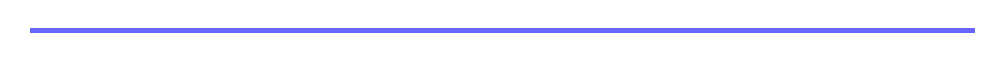
\begin{tikzpicture}
        \draw[line width=2pt, color=blue!60] (0,0) -- (12,0);
    \end{tikzpicture}
    
    \vspace{1.5cm}
    
    {\Large Technical Documentation\par}
    
    \vspace{3cm}
    
    {\large
    \begin{tabular}{rl}
        \textbf{Version:} & 1.0 \\[0.3cm]
        \textbf{Date:} & \today \\
    \end{tabular}
    \par}
    
    \vfill
    
    {\large Machine Learning Pipeline Documentation\par}
    {\normalsize From Data Collection to Production Deployment\par}
    
\end{titlepage}

\begin{abstract}
This document provides a comprehensive technical overview of the BikeFit AI system, an end-to-end machine learning pipeline for analyzing cycling posture and bike angles from video footage. The system comprises four main components: a dataset creation tool for synchronizing video with IMU sensor data, a deep learning model for bike angle prediction, a real-time joint angle detection system, and a web application for user-facing video analysis. This documentation explains the architecture, data flow, and implementation details of each component.
\end{abstract}

\tableofcontents
\newpage

% ============================================================================
\section{System Overview}
% ============================================================================

The BikeFit AI system is designed to analyze cycling videos and provide objective measurements of rider posture and bike orientation. The system leverages computer vision and deep learning to:

\begin{itemize}
    \item Detect and track the cyclist's body joints (shoulders, elbows, hips, knees, ankles)
    \item Calculate joint angles (knee flexion, hip angle, elbow angle)
    \item Segment the bicycle from the video frame
    \item Predict the bike's tilt angle relative to the camera
\end{itemize}

\subsection{Repository Structure}

The codebase is organized into the following main directories:

\begin{table}[H]
\centering
\begin{tabular}{@{}ll@{}}
\toprule
\textbf{Directory} & \textbf{Purpose} \\
\midrule
\texttt{create\_labeled\_dataset/} & GUI tool for creating training datasets \\
\texttt{bike\_angle\_detection\_model/} & Training and inference for bike angle prediction \\
\texttt{joint\_angle\_detection/} & Real-time webcam-based joint angle detection \\
\texttt{bikefitting-web/} & Production web application (frontend + backend) \\
\texttt{sam3/} & External segmentation model (SAM3, installed editable) \\
\bottomrule
\end{tabular}
\caption{Main directory structure of the BikeFit AI repository}
\end{table}

\subsection{System Architecture}

Figure~\ref{fig:architecture} illustrates the high-level architecture of the complete system, showing both the offline training pipeline (left) and the online inference pipeline (right). The trained ConvNeXt model bridges these two phases.

\begin{figure}[H]
\centering
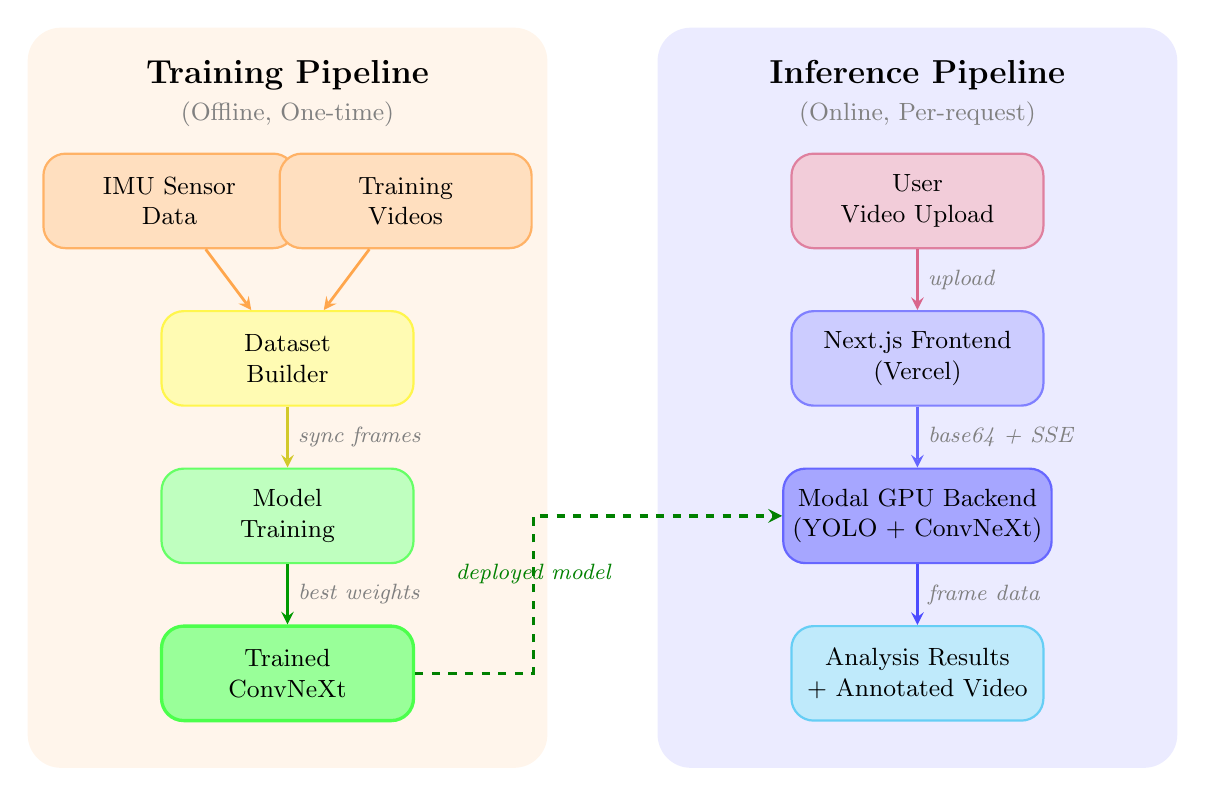
\begin{tikzpicture}[
    node distance=1.8cm,
    box/.style={rectangle, draw, rounded corners=8pt, minimum width=3.2cm, minimum height=1.2cm, align=center, font=\small, line width=0.8pt},
    arrow/.style={->, thick, >=stealth, line width=1pt},
    label/.style={font=\footnotesize\itshape, text=gray}
]

% ==================== TRAINING PIPELINE (Left) ====================
% Background box for training
\begin{scope}[on background layer]
    \fill[orange!8, rounded corners=12pt] (-1.8,1.2) rectangle (4.8,-8.2);
\end{scope}

% Title
\node[font=\bfseries\large] at (1.5, 0.6) {Training Pipeline};
\node[font=\small, text=gray] at (1.5, 0.1) {(Offline, One-time)};

% Nodes
\node[box, fill=orange!25, draw=orange!60] (imu) at (0, -1) {IMU Sensor\\Data};
\node[box, fill=orange!25, draw=orange!60] (video) at (3, -1) {Training\\Videos};
\node[box, fill=yellow!30, draw=yellow!70] (dataset) at (1.5, -3) {Dataset\\Builder};
\node[box, fill=green!25, draw=green!60] (train) at (1.5, -5) {Model\\Training};
\node[box, fill=green!40, draw=green!70, line width=1.2pt] (model) at (1.5, -7) {Trained\\ConvNeXt};

% Arrows with labels
\draw[arrow, color=orange!70] (imu) -- (dataset);
\draw[arrow, color=orange!70] (video) -- (dataset);
\draw[arrow, color=yellow!80!black] (dataset) -- node[right, label] {sync frames} (train);
\draw[arrow, color=green!60!black] (train) -- node[right, label] {best weights} (model);

% ==================== INFERENCE PIPELINE (Right) ====================
% Background box for inference
\begin{scope}[on background layer]
    \fill[blue!8, rounded corners=12pt] (6.2,1.2) rectangle (12.8,-8.2);
\end{scope}

% Title
\node[font=\bfseries\large] at (9.5, 0.6) {Inference Pipeline};
\node[font=\small, text=gray] at (9.5, 0.1) {(Online, Per-request)};

% Nodes
\node[box, fill=purple!20, draw=purple!50] (user) at (9.5, -1) {User\\Video Upload};
\node[box, fill=blue!20, draw=blue!50] (frontend) at (9.5, -3) {Next.js Frontend\\(Vercel)};
\node[box, fill=blue!35, draw=blue!60] (modal) at (9.5, -5) {Modal GPU Backend\\(YOLO + ConvNeXt)};
\node[box, fill=cyan!25, draw=cyan!60] (results) at (9.5, -7) {Analysis Results\\+ Annotated Video};

% Arrows with labels
\draw[arrow, color=purple!60] (user) -- node[right, label] {upload} (frontend);
\draw[arrow, color=blue!60] (frontend) -- node[right, label] {base64 + SSE} (modal);
\draw[arrow, color=blue!70] (modal) -- node[right, label] {frame data} (results);

% ==================== MODEL TRANSFER ====================
% Dashed arrow from trained model to inference
\draw[arrow, dashed, color=green!50!black, line width=1.2pt] 
    (model.east) -- ++(1.5,0) |- node[above, pos=0.25, font=\footnotesize\itshape, text=green!50!black] {deployed model} (modal.west);

\end{tikzpicture}
\caption{System architecture overview. \textbf{Left:} The training pipeline creates labeled data from video-IMU synchronization and trains the angle classifier. \textbf{Right:} The inference pipeline processes user videos in real-time on cloud GPUs. The trained model (dashed arrow) connects both pipelines.}
\label{fig:architecture}
\end{figure}

% ============================================================================
\section{Dataset Creation (\texttt{create\_labeled\_dataset/})}
% ============================================================================

The dataset creation module provides a graphical user interface (GUI) for synchronizing video recordings with IMU (Inertial Measurement Unit) sensor data to create labeled training datasets.

\subsection{Purpose}

To train a model that predicts bike angles, we need ground truth labels. These labels come from an IMU sensor attached to the bicycle that records the actual orientation. The challenge is synchronizing the video frames with the IMU timestamps.

\subsection{Input Requirements}

\begin{itemize}
    \item \textbf{Videos}: Cycling footage placed in \texttt{create\_labeled\_dataset/videos/}
    \item \textbf{IMU Data}: CSV files from the IMU sensor in \texttt{create\_labeled\_dataset/imu\_runs/}
\end{itemize}

\subsection{Synchronization Process}

The synchronization workflow involves:

\begin{enumerate}
    \item \textbf{Video Selection}: User selects a video file from the interface
    \item \textbf{Time Reference}: User identifies a frame where a clock/phone time is visible
    \item \textbf{IMU Matching}: The system automatically finds the corresponding IMU recording based on the timestamp
    \item \textbf{Sync Point}: User marks the exact frame that corresponds to the IMU start time
    \item \textbf{Trim Points}: Optional start/end trim points to exclude unusable footage
\end{enumerate}

\subsection{Output Format}

The tool generates:

\begin{itemize}
    \item \texttt{synchronized\_dataset.csv}: Contains frame paths and corresponding bike angles
    \item \texttt{frames/}: Directory of extracted video frames
\end{itemize}

\begin{table}[H]
\centering
\begin{tabular}{@{}lll@{}}
\toprule
\textbf{Column} & \textbf{Type} & \textbf{Description} \\
\midrule
\texttt{frame\_path} & string & Relative path to the extracted frame image \\
\texttt{bike\_angle\_deg} & float & Ground truth angle in degrees $[-180, 180]$ \\
\texttt{sync\_time\_diff\_ms} & float & Synchronization quality metric \\
\bottomrule
\end{tabular}
\caption{Output CSV schema for the synchronized dataset}
\end{table}

\subsection{Key Files}

\begin{itemize}
    \item \texttt{1\_build\_dataset.py}: Main entry point, launches the GUI
    \item \texttt{dataset\_builder.py}: Core logic for video-IMU synchronization
\end{itemize}

% ============================================================================
\section{Bike Angle Detection Model (\texttt{bike\_angle\_detection\_model/})}
% ============================================================================

This module implements the deep learning pipeline for predicting the camera-relative bike angle from video frames.

\subsection{Model Architecture}

The bike angle prediction uses a two-stage approach:

\begin{enumerate}
    \item \textbf{Bike Segmentation}: YOLOv8n-seg isolates the bicycle pixels
    \item \textbf{Angle Classification}: ConvNeXt-Tiny classifies the masked bike image into angle bins
\end{enumerate}

\subsubsection{Why Classification over Regression?}

Angle prediction is formulated as a classification problem rather than regression because:

\begin{itemize}
    \item Angles are circular: $-180°$ and $+180°$ are the same orientation
    \item Classification with soft labels naturally handles circular wrap-around
    \item The model outputs a probability distribution, enabling uncertainty estimation
\end{itemize}

\subsection{Circular Soft Labels}

\subsubsection{The Problem with Standard Labels}

Consider a bike at $179°$. With standard one-hot labels, the model learns that $179°$ is ``correct'' and all other angles are equally wrong. But intuitively:
\begin{itemize}
    \item $178°$ should be \textit{almost} correct (only $1°$ error)
    \item $-179°$ should \textit{also} be almost correct (only $2°$ away, wrapping around the circle!)
    \item $0°$ should be very wrong ($179°$ error)
\end{itemize}

Standard regression also fails because it doesn't understand that $-180°$ and $+180°$ represent the \textit{same} physical orientation.

\subsubsection{The Solution: Circular Gaussian Soft Labels}

Instead of assigning 100\% probability to a single bin, we spread the probability across nearby bins using a Gaussian distribution that \textbf{wraps around the circle}. This teaches the model that nearby angles are similar, even across the $\pm 180°$ boundary.

\begin{figure}[H]
\centering
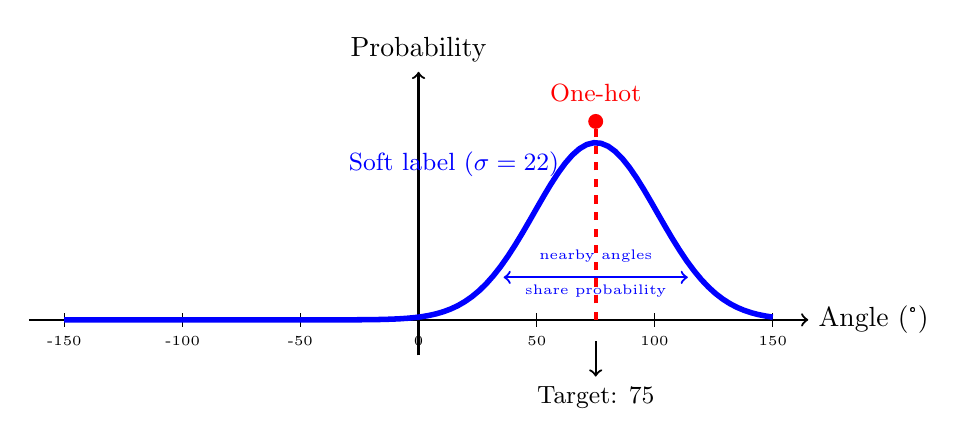
\begin{tikzpicture}[scale=0.9]
    % Draw the angle axis
    \draw[thick, ->] (-5.5,0) -- (5.5,0) node[right] {Angle (°)};
    \draw[thick, ->] (0,-0.5) -- (0,3.5) node[above] {Probability};
    
    % Tick marks
    \foreach \x/\label in {-5/-150, -3.33/-100, -1.67/-50, 0/0, 1.67/50, 3.33/100, 5/150} {
        \draw (\x, -0.1) -- (\x, 0.1);
        \node[below, font=\tiny] at (\x, -0.1) {\label};
    }
    
    % Standard one-hot label (red, dashed)
    \draw[red, dashed, line width=1.5pt] (2.5, 0) -- (2.5, 2.8);
    \node[red, font=\small] at (2.5, 3.2) {One-hot};
    \fill[red] (2.5, 2.8) circle (3pt);
    
    % Soft Gaussian label (blue, solid) - centered at 75°
    \draw[blue, line width=2pt, domain=-5:5, samples=100] 
        plot (\x, {2.5*exp(-(\x-2.5)^2/1.5)});
    \node[blue, font=\small] at (0.5, 2.2) {Soft label ($\sigma=22°$)};
    
    % Highlight the target angle
    \draw[<-, thick] (2.5, -0.8) -- (2.5, -0.3);
    \node[font=\small] at (2.5, -1.1) {Target: $75°$};
    
    % Show that nearby bins get probability
    \draw[blue, <->, thick] (1.2, 0.6) -- (3.8, 0.6);
    \node[blue, font=\tiny] at (2.5, 0.9) {nearby angles};
    \node[blue, font=\tiny] at (2.5, 0.4) {share probability};
\end{tikzpicture}
\caption{Comparison of one-hot labels (red spike) vs.\ circular soft labels (blue curve). Soft labels assign partial probability to neighboring bins, teaching the model that $73°$ and $77°$ are almost as correct as $75°$.}
\label{fig:softlabels}
\end{figure}

\subsubsection{Mathematical Formulation}

The angle space $[-180°, +180°]$ is divided into $N$ bins (default: $N=120$, giving $3°$ per bin). For a ground truth angle $\theta$, the soft label probability for bin $i$ with center $c_i$ is:

\begin{equation}
    p_i = \frac{1}{Z} \exp\left(-\frac{d_{\text{circ}}(\theta, c_i)^2}{2\sigma^2}\right)
\end{equation}

The key is the \textbf{circular distance} function, which measures the shortest path around the circle:

\begin{equation}
    d_{\text{circ}}(\theta_1, \theta_2) = \text{atan2}\big(\sin(\theta_1 - \theta_2), \cos(\theta_1 - \theta_2)\big)
\end{equation}

This ensures that $d_{\text{circ}}(-179°, +179°) = 2°$, not $358°$. The normalization constant $Z = \sum_i \exp(\cdot)$ ensures probabilities sum to 1.

\paragraph{Intuition:} The smoothing parameter $\sigma = 22°$ means bins within $\sim 22°$ of the true angle receive significant probability. This makes the model robust to small labeling errors and encourages learning continuous angle representations.

\subsection{Prediction via Circular Mean}

At inference time, the model outputs a probability distribution over all bins. To convert this back to a single angle prediction, we compute the \textbf{circular mean}:

\begin{equation}
    \hat{\theta} = \text{atan2}\left(\sum_i p_i \sin(c_i), \sum_i p_i \cos(c_i)\right)
\end{equation}

\paragraph{Why not just take argmax?} The argmax would give the single highest-probability bin. The circular mean is better because:
\begin{enumerate}
    \item It uses information from \textit{all} bins, not just the peak
    \item It correctly handles wrap-around (if probability is split between $-179°$ and $+179°$, the mean is $180°$, not $0°$)
    \item It provides sub-bin precision (can predict $74.3°$, not just bin centers)
\end{enumerate}

\subsection{Training Pipeline}

\begin{enumerate}
    \item \textbf{Preprocessing} (\texttt{1\_preprocess.py}):
    \begin{itemize}
        \item Load each frame from the dataset
        \item Run YOLOv8n-seg to detect and mask the bicycle
        \item Crop to a square region around the bike
        \item Resize to $224 \times 224$ pixels
        \item Save masked images to \texttt{data/frames/}
    \end{itemize}
    
    \item \textbf{Training} (\texttt{2\_train.py}):
    \begin{itemize}
        \item Load masked images with corresponding angle labels
        \item Split into training (80\%) and validation (20\%) sets
        \item Train ConvNeXt-Tiny backbone with custom classification head
        \item Use cross-entropy loss against soft labels
        \item Save best model based on validation MAE
    \end{itemize}
    
    \item \textbf{Inference} (\texttt{3\_inference.py}):
    \begin{itemize}
        \item Load trained model
        \item Process single images or batch CSV files
        \item Output predicted angles with confidence scores
    \end{itemize}
\end{enumerate}

\subsection{Hyperparameters}

The following hyperparameters were optimized via Optuna search:

\begin{table}[H]
\centering
\begin{tabular}{@{}llr@{}}
\toprule
\textbf{Parameter} & \textbf{Description} & \textbf{Value} \\
\midrule
Backbone & CNN architecture & ConvNeXt-Tiny \\
Number of bins & Angle discretization & 120 (3° per bin) \\
Label smoothing ($\sigma$) & Gaussian spread & 22° \\
Learning rate & Adam optimizer & $3.4 \times 10^{-5}$ \\
Batch size & Training batch size & 48 \\
Epochs & Maximum training epochs & 100 \\
\bottomrule
\end{tabular}
\caption{Optimized hyperparameters for bike angle classification}
\end{table}

\subsection{Performance}

The model achieves approximately \textbf{2° Mean Absolute Error (MAE)} on the validation set.

% ============================================================================
\section{Joint Angle Detection (\texttt{joint\_angle\_detection/})}
% ============================================================================

This module provides real-time joint angle detection from a webcam feed using YOLOv8 pose estimation.

\subsection{Functionality}

The system:

\begin{enumerate}
    \item Captures frames from a webcam or video source
    \item Runs YOLOv8m-pose to detect 17 body keypoints
    \item Calculates three primary joint angles on the detected side
    \item Overlays the skeleton and angle measurements on the video
\end{enumerate}

\subsection{Measured Angles}

\begin{table}[H]
\centering
\begin{tabular}{@{}lll@{}}
\toprule
\textbf{Angle} & \textbf{Joints Involved} & \textbf{Significance} \\
\midrule
Knee angle & Hip → Knee → Ankle & Pedaling efficiency, saddle height \\
Hip angle & Shoulder → Hip → Knee & Torso position, aerodynamics \\
Elbow angle & Shoulder → Elbow → Wrist & Arm position, handlebar reach \\
\bottomrule
\end{tabular}
\caption{Joint angles calculated by the detection system}
\end{table}

\subsection{Angle Calculation}

For three points $A$, $B$, $C$, the angle $\angle ABC$ is calculated as:

\begin{equation}
    \angle ABC = \arccos\left(\frac{\vec{BA} \cdot \vec{BC}}{|\vec{BA}| \cdot |\vec{BC}|}\right)
\end{equation}

where $\vec{BA} = A - B$ and $\vec{BC} = C - B$.

\subsection{Side Detection}

The system automatically determines whether the left or right side of the body is facing the camera by counting visible keypoints on each side. The side with more high-confidence keypoints is selected for angle calculation.

\subsection{Usage}

\begin{lstlisting}[style=code, language=bash]
cd joint_angle_detection
python 1_live_camera.py --source 0 --min_conf 0.5
\end{lstlisting}

Options:
\begin{itemize}
    \item \texttt{--source}: Camera index (0 for default webcam)
    \item \texttt{--side}: Force left/right side (default: auto)
    \item \texttt{--min\_conf}: Minimum keypoint confidence threshold
\end{itemize}

% ============================================================================
\section{Web Application (\texttt{bikefitting-web/})}
% ============================================================================

The web application provides a user-friendly interface for video analysis, combining all AI models into a single production-ready service.

\subsection{Architecture Overview}

\begin{figure}[H]
\centering
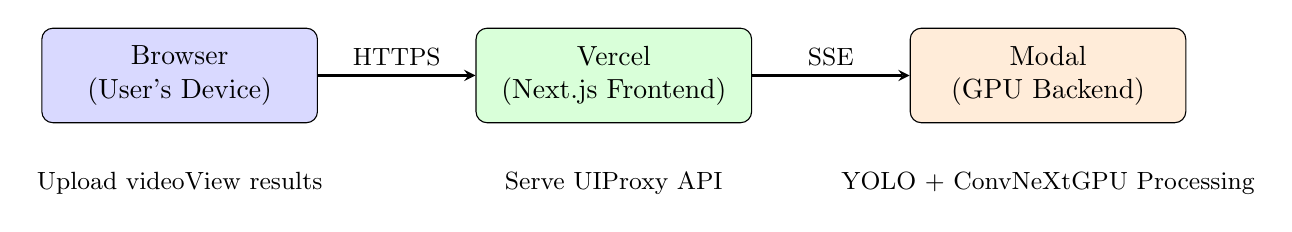
\begin{tikzpicture}[
    node distance=2cm,
    box/.style={rectangle, draw, rounded corners, minimum width=3.5cm, minimum height=1.2cm, align=center},
    arrow/.style={->, thick, >=stealth}
]

\node[box, fill=blue!15] (browser) {Browser\\(User's Device)};
\node[box, fill=green!15, right=of browser] (vercel) {Vercel\\(Next.js Frontend)};
\node[box, fill=orange!15, right=of vercel] (modal) {Modal\\(GPU Backend)};

\draw[arrow] (browser) -- node[above, font=\small] {HTTPS} (vercel);
\draw[arrow] (vercel) -- node[above, font=\small] {SSE} (modal);

\node[below=0.5cm of browser, font=\small] {Upload video\\View results};
\node[below=0.5cm of vercel, font=\small] {Serve UI\\Proxy API};
\node[below=0.5cm of modal, font=\small] {YOLO + ConvNeXt\\GPU Processing};

\end{tikzpicture}
\caption{Web application architecture}
\end{figure}

\subsection{Frontend (\texttt{bikefitting-web/frontend/})}

The frontend is built with \textbf{Next.js 15} and \textbf{React 19}, deployed on Vercel.

\subsubsection{Key Components}

\begin{itemize}
    \item \texttt{src/app/page.tsx}: Main application page, orchestrates the upload and results flow
    \item \texttt{src/components/VideoUploader.tsx}: Handles file selection, preview, settings, and upload progress
    \item \texttt{src/components/ResultsViewer.tsx}: Displays processed video with synchronized live angle data
\end{itemize}

\subsubsection{Features}

\begin{itemize}
    \item Drag-and-drop video upload
    \item Time range selection with visual timeline
    \item Adjustable output FPS (5-30)
    \item Real-time processing progress via Server-Sent Events (SSE)
    \item Synchronized live angle display during video playback
    \item Video download capability
\end{itemize}

\subsubsection{Technology Stack}

\begin{table}[H]
\centering
\begin{tabular}{@{}ll@{}}
\toprule
\textbf{Technology} & \textbf{Purpose} \\
\midrule
Next.js 15 & React framework with App Router \\
React 19 & UI component library \\
TypeScript & Type-safe JavaScript \\
Tailwind CSS & Utility-first styling \\
Lucide React & Icon library \\
\bottomrule
\end{tabular}
\caption{Frontend technology stack}
\end{table}

\subsection{Backend (\texttt{bikefitting-web/backend/})}

The backend runs on \textbf{Modal}, a serverless GPU platform that provides on-demand NVIDIA T4 GPUs.

\subsubsection{Key Files}

\begin{itemize}
    \item \texttt{modal\_app.py}: Main application defining all API endpoints
    \item \texttt{processing/}: Processing modules (bike segmenter, angle predictor, pose detector, video processor)
\end{itemize}

\subsubsection{API Endpoints}

\begin{table}[H]
\centering
\begin{tabular}{@{}llp{7cm}@{}}
\toprule
\textbf{Endpoint} & \textbf{Method} & \textbf{Description} \\
\midrule
\texttt{/process\_video\_stream} & POST & Accepts base64-encoded video, returns SSE stream with progress updates and final results \\
\texttt{/download} & GET & Returns the processed video file by job ID \\
\texttt{/health} & GET & Health check and system limits \\
\bottomrule
\end{tabular}
\caption{Backend API endpoints}
\end{table}

\subsubsection{Processing Pipeline}

For each uploaded video, the backend:

\begin{enumerate}
    \item Decodes the base64 video and saves to temporary storage
    \item Loads the three AI models (YOLOv8-seg, YOLOv8-pose, ConvNeXt)
    \item For each frame:
    \begin{enumerate}
        \item Detect human pose and calculate joint angles
        \item Segment the bicycle and predict tilt angle
        \item Store per-frame angle data
        \item Draw skeleton overlay on the output frame
    \end{enumerate}
    \item Encode output video with H.264 codec (FFmpeg)
    \item Return frame-by-frame angle data to frontend
\end{enumerate}

\subsubsection{AI Models Used}

\begin{table}[H]
\centering
\begin{tabular}{@{}llp{6cm}@{}}
\toprule
\textbf{Model} & \textbf{Task} & \textbf{Output} \\
\midrule
YOLOv8n-seg & Instance segmentation & Bicycle pixel mask \\
YOLOv8m-pose & Pose estimation & 17 body keypoints with confidence \\
ConvNeXt-Tiny & Angle classification & Bike tilt angle $[-180°, 180°]$ \\
\bottomrule
\end{tabular}
\caption{AI models in the processing pipeline}
\end{table}

\subsection{Data Flow}

\begin{enumerate}
    \item \textbf{Upload}: User selects video → Browser reads as base64 → Direct POST to Modal endpoint
    \item \textbf{Processing}: Modal GPU processes video → Streams progress via SSE
    \item \textbf{Results}: 
    \begin{itemize}
        \item \texttt{frame\_data}: Array of per-frame angles (JSON)
        \item \texttt{job\_id}: Identifier for video download
    \end{itemize}
    \item \textbf{Playback}: Video loads from Modal → Frontend syncs current playback time with \texttt{frame\_data} to display live angles
\end{enumerate}

\subsection{Security Measures}

The application implements several security measures:

\begin{itemize}
    \item \textbf{Input Validation}: File size limits (200MB), duration limits (2 minutes), FPS range enforcement
    \item \textbf{Path Traversal Prevention}: Job IDs are sanitized to alphanumeric characters only
    \item \textbf{Security Headers}: X-Frame-Options, X-Content-Type-Options, Referrer-Policy, Permissions-Policy
    \item \textbf{Rate Limiting}: 10 requests per hour per client
    \item \textbf{Temp File Cleanup}: Input files are deleted after processing
\end{itemize}

\subsection{Deployment}

\subsubsection{Backend Deployment (Modal)}

\begin{lstlisting}[style=code, language=bash]
# Install Modal CLI
pip install modal

# Authenticate
modal setup

# Create persistent volume for model
modal volume create bikefitting-models
modal volume put bikefitting-models best_model.pt best_model.pt

# Deploy
cd bikefitting-web/backend
modal deploy modal_app.py
\end{lstlisting}

\subsubsection{Frontend Deployment (Vercel)}

\begin{lstlisting}[style=code, language=bash]
cd bikefitting-web/frontend
npm install
vercel

# Set environment variables in Vercel dashboard:
# NEXT_PUBLIC_MODAL_STREAM_URL
# NEXT_PUBLIC_MODAL_DOWNLOAD_URL
\end{lstlisting}

% ============================================================================
\section{Dependencies and External Packages}
% ============================================================================

\subsection{Python Dependencies}

\begin{table}[H]
\centering
\begin{tabular}{@{}lll@{}}
\toprule
\textbf{Package} & \textbf{Version} & \textbf{Purpose} \\
\midrule
PyTorch & $\geq$ 2.0.0 & Deep learning framework \\
torchvision & $\geq$ 0.15.0 & Image transforms and pretrained models \\
ultralytics & $\geq$ 8.0.0 & YOLOv8 models (seg, pose) \\
opencv-python & $\geq$ 4.8.0 & Image and video processing \\
numpy & $\geq$ 1.24.0 & Numerical operations \\
pandas & --- & Data manipulation \\
tqdm & $\geq$ 4.65.0 & Progress bars \\
Pillow & $\geq$ 10.0.0 & Image I/O \\
\bottomrule
\end{tabular}
\caption{Core Python dependencies}
\end{table}

\subsection{SAM3 (\texttt{sam3/})}

The SAM3 directory contains Meta's Segment Anything Model 3, installed in editable mode. This package provides advanced segmentation capabilities and is included as a Git submodule.

% ============================================================================
\section{Conclusion}
% ============================================================================

The BikeFit AI system demonstrates an end-to-end machine learning pipeline from data collection to production deployment. Key technical achievements include:

\begin{itemize}
    \item \textbf{Novel angle representation}: Circular soft labels with Gaussian smoothing for handling angular wrap-around
    \item \textbf{Multi-model inference}: Combining segmentation, pose estimation, and classification in a single pipeline
    \item \textbf{Real-time synchronization}: Frame-accurate angle display synchronized with video playback
    \item \textbf{Serverless GPU deployment}: Cost-effective on-demand GPU processing via Modal
\end{itemize}

The system achieves approximately 2° mean absolute error for bike angle prediction while providing real-time joint angle measurements for comprehensive cycling posture analysis.

% ============================================================================
\appendix
\section{File Reference}
% ============================================================================

\begin{table}[H]
\centering
\small
\begin{tabular}{@{}lp{9cm}@{}}
\toprule
\textbf{File} & \textbf{Description} \\
\midrule
\multicolumn{2}{l}{\textit{create\_labeled\_dataset/}} \\
\texttt{1\_build\_dataset.py} & Main entry point for dataset builder GUI \\
\texttt{dataset\_builder.py} & Core synchronization logic \\
\midrule
\multicolumn{2}{l}{\textit{bike\_angle\_detection\_model/}} \\
\texttt{1\_preprocess.py} & Masks bikes and creates training data \\
\texttt{2\_train.py} & Trains the ConvNeXt angle classifier \\
\texttt{3\_inference.py} & Runs inference on new images \\
\texttt{generate\_demo\_video.py} & Creates annotated demo videos \\
\midrule
\multicolumn{2}{l}{\textit{joint\_angle\_detection/}} \\
\texttt{1\_live\_camera.py} & Real-time webcam angle detection \\
\texttt{core.py} & Pose detection and angle calculation functions \\
\midrule
\multicolumn{2}{l}{\textit{bikefitting-web/backend/}} \\
\texttt{modal\_app.py} & Modal serverless API endpoints \\
\texttt{processing/*.py} & Video processing modules \\
\midrule
\multicolumn{2}{l}{\textit{bikefitting-web/frontend/src/}} \\
\texttt{app/page.tsx} & Main application page \\
\texttt{components/VideoUploader.tsx} & Video upload interface \\
\texttt{components/ResultsViewer.tsx} & Results display interface \\
\bottomrule
\end{tabular}
\caption{Complete file reference}
\end{table}

\end{document}

